% Created by tikzDevice version 0.10.1 on 2016-11-18 13:51:07
% !TEX encoding = UTF-8 Unicode
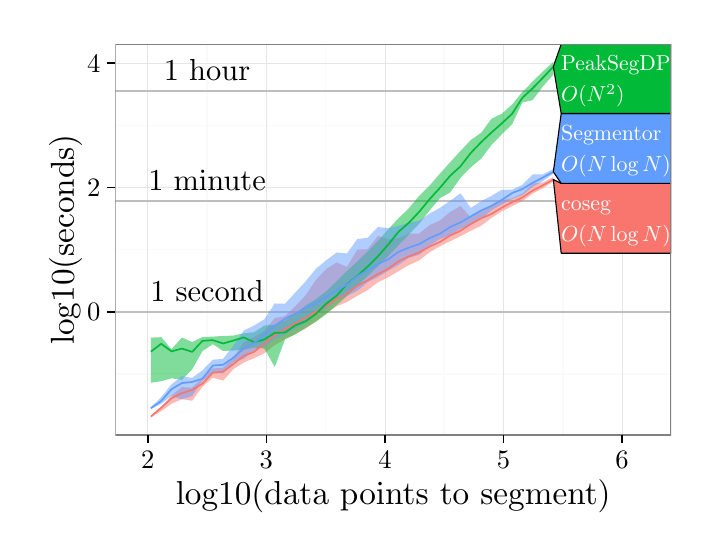
\begin{tikzpicture}[x=1pt,y=1pt]
\definecolor{fillColor}{RGB}{255,255,255}
\path[use as bounding box,fill=fillColor,fill opacity=0.00] (0,0) rectangle (238.49,180.67);
\begin{scope}
\path[clip] (  0.00,  0.00) rectangle (238.49,180.67);
\definecolor{drawColor}{RGB}{255,255,255}
\definecolor{fillColor}{RGB}{255,255,255}

\path[draw=drawColor,line width= 0.6pt,line join=round,line cap=round,fill=fillColor] (  0.00,  0.00) rectangle (238.49,180.68);
\end{scope}
\begin{scope}
\path[clip] ( 31.66, 33.48) rectangle (232.49,174.67);
\definecolor{fillColor}{RGB}{255,255,255}

\path[fill=fillColor] ( 31.66, 33.48) rectangle (232.49,174.67);
\definecolor{drawColor}{gray}{0.98}

\path[draw=drawColor,line width= 0.6pt,line join=round] ( 31.66, 55.58) --
	(232.49, 55.58);

\path[draw=drawColor,line width= 0.6pt,line join=round] ( 31.66,100.48) --
	(232.49,100.48);

\path[draw=drawColor,line width= 0.6pt,line join=round] ( 31.66,145.37) --
	(232.49,145.37);

\path[draw=drawColor,line width= 0.6pt,line join=round] ( 64.81, 33.48) --
	( 64.81,174.67);

\path[draw=drawColor,line width= 0.6pt,line join=round] (107.66, 33.48) --
	(107.66,174.67);

\path[draw=drawColor,line width= 0.6pt,line join=round] (150.51, 33.48) --
	(150.51,174.67);

\path[draw=drawColor,line width= 0.6pt,line join=round] (193.37, 33.48) --
	(193.37,174.67);
\definecolor{drawColor}{gray}{0.90}

\path[draw=drawColor,line width= 0.2pt,line join=round] ( 31.66, 78.03) --
	(232.49, 78.03);

\path[draw=drawColor,line width= 0.2pt,line join=round] ( 31.66,122.92) --
	(232.49,122.92);

\path[draw=drawColor,line width= 0.2pt,line join=round] ( 31.66,167.81) --
	(232.49,167.81);

\path[draw=drawColor,line width= 0.2pt,line join=round] ( 43.38, 33.48) --
	( 43.38,174.67);

\path[draw=drawColor,line width= 0.2pt,line join=round] ( 86.24, 33.48) --
	( 86.24,174.67);

\path[draw=drawColor,line width= 0.2pt,line join=round] (129.09, 33.48) --
	(129.09,174.67);

\path[draw=drawColor,line width= 0.2pt,line join=round] (171.94, 33.48) --
	(171.94,174.67);

\path[draw=drawColor,line width= 0.2pt,line join=round] (214.79, 33.48) --
	(214.79,174.67);
\definecolor{drawColor}{RGB}{190,190,190}

\path[draw=drawColor,line width= 0.6pt,line join=round] ( 31.66, 78.03) -- (232.49, 78.03);

\path[draw=drawColor,line width= 0.6pt,line join=round] ( 31.66,117.94) -- (232.49,117.94);

\path[draw=drawColor,line width= 0.6pt,line join=round] ( 31.66,157.85) -- (232.49,157.85);
\definecolor{fillColor}{RGB}{248,118,109}

\path[fill=fillColor,fill opacity=0.50] ( 44.52, 40.37) --
	( 48.25, 43.52) --
	( 51.98, 47.80) --
	( 55.71, 50.77) --
	( 59.44, 50.60) --
	( 63.17, 54.11) --
	( 66.89, 57.52) --
	( 70.62, 57.76) --
	( 74.35, 61.42) --
	( 78.08, 67.01) --
	( 81.81, 68.90) --
	( 85.54, 71.19) --
	( 89.27, 75.73) --
	( 93.00, 76.43) --
	( 96.73, 80.07) --
	(100.45, 83.97) --
	(104.18, 89.56) --
	(107.91, 93.48) --
	(111.64, 95.84) --
	(115.37, 94.23) --
	(119.10,100.44) --
	(122.83,100.62) --
	(126.56,105.44) --
	(130.29,104.14) --
	(134.01,104.61) --
	(137.74,106.25) --
	(141.47,106.27) --
	(145.20,109.31) --
	(148.93,110.98) --
	(152.66,114.08) --
	(156.39,116.25) --
	(160.12,112.06) --
	(163.85,114.58) --
	(167.57,116.49) --
	(171.30,118.39) --
	(175.03,119.01) --
	(178.76,120.74) --
	(182.49,124.34) --
	(186.22,124.77) --
	(189.95,126.66) --
	(189.95,125.10) --
	(186.22,122.65) --
	(182.49,120.74) --
	(178.76,117.99) --
	(175.03,116.16) --
	(171.30,114.30) --
	(167.57,111.90) --
	(163.85,109.10) --
	(160.12,107.29) --
	(156.39,105.30) --
	(152.66,103.50) --
	(148.93,101.68) --
	(145.20, 99.50) --
	(141.47, 96.58) --
	(137.74, 94.87) --
	(134.01, 92.69) --
	(130.29, 90.49) --
	(126.56, 88.64) --
	(122.83, 85.83) --
	(119.10, 83.79) --
	(115.37, 81.54) --
	(111.64, 79.98) --
	(107.91, 77.51) --
	(104.18, 74.55) --
	(100.45, 71.95) --
	( 96.73, 69.98) --
	( 93.00, 68.12) --
	( 89.27, 65.96) --
	( 85.54, 63.05) --
	( 81.81, 61.26) --
	( 78.08, 59.67) --
	( 74.35, 57.28) --
	( 70.62, 53.16) --
	( 66.89, 54.23) --
	( 63.17, 50.92) --
	( 59.44, 45.89) --
	( 55.71, 46.40) --
	( 51.98, 44.78) --
	( 48.25, 42.07) --
	( 44.52, 39.89) --
	cycle;
\definecolor{fillColor}{RGB}{0,186,56}

\path[fill=fillColor,fill opacity=0.50] ( 44.52, 68.67) --
	( 48.25, 68.83) --
	( 51.98, 64.48) --
	( 55.71, 68.70) --
	( 59.44, 67.07) --
	( 63.17, 68.88) --
	( 66.89, 69.02) --
	( 70.62, 69.29) --
	( 74.35, 69.39) --
	( 78.08, 70.25) --
	( 81.81, 70.61) --
	( 85.54, 73.02) --
	( 89.27, 73.31) --
	( 93.00, 74.84) --
	( 96.73, 77.47) --
	(100.45, 80.24) --
	(104.18, 82.60) --
	(107.91, 85.45) --
	(111.64, 89.07) --
	(115.37, 92.74) --
	(119.10, 96.17) --
	(122.83, 99.78) --
	(126.56,103.57) --
	(130.29,107.82) --
	(134.01,111.83) --
	(137.74,115.38) --
	(141.47,119.91) --
	(145.20,123.57) --
	(148.93,127.89) --
	(152.66,132.04) --
	(156.39,136.12) --
	(160.12,140.08) --
	(163.85,142.67) --
	(167.57,147.74) --
	(171.30,149.55) --
	(175.03,152.88) --
	(178.76,157.44) --
	(182.49,161.21) --
	(186.22,164.92) --
	(189.95,168.26) --
	(189.95,163.69) --
	(186.22,159.51) --
	(182.49,154.50) --
	(178.76,153.65) --
	(175.03,145.76) --
	(171.30,142.09) --
	(167.57,138.25) --
	(163.85,133.32) --
	(160.12,130.23) --
	(156.39,126.41) --
	(152.66,121.11) --
	(148.93,119.03) --
	(145.20,114.55) --
	(141.47,109.81) --
	(137.74,105.92) --
	(134.01,102.05) --
	(130.29, 98.15) --
	(126.56, 94.50) --
	(122.83, 90.89) --
	(119.10, 87.40) --
	(115.37, 83.70) --
	(111.64, 80.44) --
	(107.91, 77.14) --
	(104.18, 74.44) --
	(100.45, 72.20) --
	( 96.73, 69.87) --
	( 93.00, 68.07) --
	( 89.27, 58.07) --
	( 85.54, 64.71) --
	( 81.81, 65.08) --
	( 78.08, 64.28) --
	( 74.35, 64.00) --
	( 70.62, 63.83) --
	( 66.89, 66.29) --
	( 63.17, 63.83) --
	( 59.44, 57.20) --
	( 55.71, 53.41) --
	( 51.98, 54.00) --
	( 48.25, 52.91) --
	( 44.52, 52.38) --
	cycle;
\definecolor{fillColor}{RGB}{97,156,255}

\path[fill=fillColor,fill opacity=0.50] ( 44.52, 43.52) --
	( 48.25, 47.13) --
	( 51.98, 51.82) --
	( 55.71, 54.66) --
	( 59.44, 54.11) --
	( 63.17, 56.86) --
	( 66.89, 60.70) --
	( 70.62, 60.98) --
	( 74.35, 65.79) --
	( 78.08, 71.23) --
	( 81.81, 73.02) --
	( 85.54, 75.30) --
	( 89.27, 81.01) --
	( 93.00, 80.91) --
	( 96.73, 84.97) --
	(100.45, 88.98) --
	(104.18, 93.58) --
	(107.91, 96.64) --
	(111.64, 99.44) --
	(115.37, 99.08) --
	(119.10,104.26) --
	(122.83,104.76) --
	(126.56,108.63) --
	(130.29,108.24) --
	(134.01,109.01) --
	(137.74,110.25) --
	(141.47,110.84) --
	(145.20,113.49) --
	(148.93,115.55) --
	(152.66,118.10) --
	(156.39,120.83) --
	(160.12,115.54) --
	(163.85,117.97) --
	(167.57,119.85) --
	(171.30,122.08) --
	(175.03,122.11) --
	(178.76,123.90) --
	(182.49,127.68) --
	(186.22,127.70) --
	(189.95,129.61) --
	(189.95,127.96) --
	(186.22,125.23) --
	(182.49,123.17) --
	(178.76,120.09) --
	(175.03,118.76) --
	(171.30,116.77) --
	(167.57,114.66) --
	(163.85,111.57) --
	(160.12,109.59) --
	(156.39,107.92) --
	(152.66,105.79) --
	(148.93,104.23) --
	(145.20,101.84) --
	(141.47, 98.63) --
	(137.74, 97.49) --
	(134.01, 94.97) --
	(130.29, 92.85) --
	(126.56, 90.61) --
	(122.83, 88.69) --
	(119.10, 85.57) --
	(115.37, 83.76) --
	(111.64, 82.21) --
	(107.91, 79.20) --
	(104.18, 77.24) --
	(100.45, 73.90) --
	( 96.73, 71.99) --
	( 93.00, 69.80) --
	( 89.27, 68.12) --
	( 85.54, 65.48) --
	( 81.81, 64.16) --
	( 78.08, 60.98) --
	( 74.35, 59.79) --
	( 70.62, 55.78) --
	( 66.89, 55.87) --
	( 63.17, 53.16) --
	( 59.44, 47.58) --
	( 55.71, 46.40) --
	( 51.98, 47.58) --
	( 48.25, 44.78) --
	( 44.52, 42.82) --
	cycle;
\definecolor{drawColor}{RGB}{248,118,109}

\path[draw=drawColor,line width= 0.6pt,line join=round] ( 44.52, 40.14) --
	( 48.25, 43.35) --
	( 51.98, 46.77) --
	( 55.71, 48.63) --
	( 59.44, 49.76) --
	( 63.17, 52.04) --
	( 66.89, 56.01) --
	( 70.62, 56.38) --
	( 74.35, 59.14) --
	( 78.08, 62.09) --
	( 81.81, 63.55) --
	( 85.54, 66.55) --
	( 89.27, 69.48) --
	( 93.00, 71.76) --
	( 96.73, 73.80) --
	(100.45, 75.85) --
	(104.18, 78.10) --
	(107.91, 80.02) --
	(111.64, 82.56) --
	(115.37, 84.63) --
	(119.10, 87.38) --
	(122.83, 89.38) --
	(126.56, 91.64) --
	(130.29, 93.54) --
	(134.01, 96.24) --
	(137.74, 98.02) --
	(141.47, 99.43) --
	(145.20,101.53) --
	(148.93,103.22) --
	(152.66,105.58) --
	(156.39,107.26) --
	(160.12,109.73) --
	(163.85,111.77) --
	(167.57,113.35) --
	(171.30,115.61) --
	(175.03,117.62) --
	(178.76,119.30) --
	(182.49,121.80) --
	(186.22,123.73) --
	(189.95,125.83);
\definecolor{drawColor}{RGB}{0,186,56}

\path[draw=drawColor,line width= 0.6pt,line join=round] ( 44.52, 63.60) --
	( 48.25, 66.44) --
	( 51.98, 63.70) --
	( 55.71, 64.71) --
	( 59.44, 63.53) --
	( 63.17, 67.51) --
	( 66.89, 67.75) --
	( 70.62, 66.55) --
	( 74.35, 67.60) --
	( 78.08, 68.75) --
	( 81.81, 67.00) --
	( 85.54, 67.99) --
	( 89.27, 70.40) --
	( 93.00, 70.51) --
	( 96.73, 73.13) --
	(100.45, 74.57) --
	(104.18, 77.23) --
	(107.91, 80.96) --
	(111.64, 83.84) --
	(115.37, 87.99) --
	(119.10, 90.94) --
	(122.83, 94.32) --
	(126.56, 98.04) --
	(130.29,102.30) --
	(134.01,106.91) --
	(137.74,110.17) --
	(141.47,114.13) --
	(145.20,118.65) --
	(148.93,122.75) --
	(152.66,127.15) --
	(156.39,130.56) --
	(160.12,135.41) --
	(163.85,139.28) --
	(167.57,142.77) --
	(171.30,146.07) --
	(175.03,149.53) --
	(178.76,155.32) --
	(182.49,158.78) --
	(186.22,162.63) --
	(189.95,166.58);
\definecolor{drawColor}{RGB}{97,156,255}

\path[draw=drawColor,line width= 0.6pt,line join=round] ( 44.52, 43.17) --
	( 48.25, 45.76) --
	( 51.98, 50.02) --
	( 55.71, 52.24) --
	( 59.44, 52.65) --
	( 63.17, 53.83) --
	( 66.89, 58.58) --
	( 70.62, 58.86) --
	( 74.35, 61.42) --
	( 78.08, 64.78) --
	( 81.81, 66.72) --
	( 85.54, 69.68) --
	( 89.27, 72.92) --
	( 93.00, 75.48) --
	( 96.73, 77.34) --
	(100.45, 79.41) --
	(104.18, 81.21) --
	(107.91, 83.45) --
	(111.64, 85.75) --
	(115.37, 87.80) --
	(119.10, 90.79) --
	(122.83, 93.03) --
	(126.56, 95.26) --
	(130.29, 96.96) --
	(134.01, 99.66) --
	(137.74,101.19) --
	(141.47,102.46) --
	(145.20,104.61) --
	(148.93,106.18) --
	(152.66,108.63) --
	(156.39,110.31) --
	(160.12,112.47) --
	(163.85,114.59) --
	(167.57,116.25) --
	(171.30,118.41) --
	(175.03,120.91) --
	(178.76,122.35) --
	(182.49,124.62) --
	(186.22,126.55) --
	(189.95,128.58);
\definecolor{drawColor}{RGB}{0,0,0}

\node[text=drawColor,anchor=base,inner sep=0pt, outer sep=0pt, scale=  1.10] at ( 64.81, 81.83) {1 second};

\node[text=drawColor,anchor=base,inner sep=0pt, outer sep=0pt, scale=  1.10] at ( 64.81,121.74) {1 minute};

\node[text=drawColor,anchor=base,inner sep=0pt, outer sep=0pt, scale=  1.10] at ( 64.81,161.66) {1 hour};
\end{scope}
\begin{scope}
\path[clip] ( 31.66, 33.48) rectangle (232.49,174.67);
\definecolor{drawColor}{RGB}{0,0,0}
\definecolor{fillColor}{RGB}{248,118,109}

\path[draw=drawColor,line width= 0.4pt,line join=round,line cap=round,fill=fillColor] (189.95,125.83) --
	(192.79,124.41) --
	(232.49,124.41) --
	(232.49, 99.15) --
	(192.79, 99.15) --
	cycle;
\definecolor{fillColor}{RGB}{97,156,255}

\path[draw=drawColor,line width= 0.4pt,line join=round,line cap=round,fill=fillColor] (189.95,128.58) --
	(192.79,149.66) --
	(232.49,149.66) --
	(232.49,124.41) --
	(192.79,124.41) --
	cycle;
\definecolor{fillColor}{RGB}{0,186,56}

\path[draw=drawColor,line width= 0.4pt,line join=round,line cap=round,fill=fillColor] (189.95,166.58) --
	(192.79,174.67) --
	(232.49,174.67) --
	(232.49,149.66) --
	(192.79,149.66) --
	cycle;
\definecolor{drawColor}{RGB}{255,255,255}

\node[text=drawColor,anchor=base west,inner sep=0pt, outer sep=0pt, scale=  0.79] at (192.79,114.75) {coseg};

\node[text=drawColor,anchor=base west,inner sep=0pt, outer sep=0pt, scale=  0.79] at (192.79,103.36) {$O(N \log N)$};

\node[text=drawColor,anchor=base west,inner sep=0pt, outer sep=0pt, scale=  0.79] at (192.79,140.01) {Segmentor};

\node[text=drawColor,anchor=base west,inner sep=0pt, outer sep=0pt, scale=  0.79] at (192.79,128.62) {$O(N \log N)$};

\node[text=drawColor,anchor=base west,inner sep=0pt, outer sep=0pt, scale=  0.78] at (192.79,165.11) {PeakSegDP};

\node[text=drawColor,anchor=base west,inner sep=0pt, outer sep=0pt, scale=  0.78] at (192.79,153.83) {$O(N^2)$};
\definecolor{drawColor}{gray}{0.50}

\path[draw=drawColor,line width= 0.6pt,line join=round,line cap=round] ( 31.66, 33.48) rectangle (232.49,174.67);
\end{scope}
\begin{scope}
\path[clip] (  0.00,  0.00) rectangle (238.49,180.67);
\definecolor{drawColor}{RGB}{0,0,0}

\node[text=drawColor,anchor=base east,inner sep=0pt, outer sep=0pt, scale=  0.96] at ( 26.26, 74.72) {0};

\node[text=drawColor,anchor=base east,inner sep=0pt, outer sep=0pt, scale=  0.96] at ( 26.26,119.62) {2};

\node[text=drawColor,anchor=base east,inner sep=0pt, outer sep=0pt, scale=  0.96] at ( 26.26,164.51) {4};
\end{scope}
\begin{scope}
\path[clip] (  0.00,  0.00) rectangle (238.49,180.67);
\definecolor{drawColor}{RGB}{0,0,0}

\path[draw=drawColor,line width= 0.6pt,line join=round] ( 28.66, 78.03) --
	( 31.66, 78.03);

\path[draw=drawColor,line width= 0.6pt,line join=round] ( 28.66,122.92) --
	( 31.66,122.92);

\path[draw=drawColor,line width= 0.6pt,line join=round] ( 28.66,167.81) --
	( 31.66,167.81);
\end{scope}
\begin{scope}
\path[clip] (  0.00,  0.00) rectangle (238.49,180.67);
\definecolor{drawColor}{RGB}{0,0,0}

\path[draw=drawColor,line width= 0.6pt,line join=round] ( 43.38, 30.48) --
	( 43.38, 33.48);

\path[draw=drawColor,line width= 0.6pt,line join=round] ( 86.24, 30.48) --
	( 86.24, 33.48);

\path[draw=drawColor,line width= 0.6pt,line join=round] (129.09, 30.48) --
	(129.09, 33.48);

\path[draw=drawColor,line width= 0.6pt,line join=round] (171.94, 30.48) --
	(171.94, 33.48);

\path[draw=drawColor,line width= 0.6pt,line join=round] (214.79, 30.48) --
	(214.79, 33.48);
\end{scope}
\begin{scope}
\path[clip] (  0.00,  0.00) rectangle (238.49,180.67);
\definecolor{drawColor}{RGB}{0,0,0}

\node[text=drawColor,anchor=base,inner sep=0pt, outer sep=0pt, scale=  0.96] at ( 43.38, 21.46) {2};

\node[text=drawColor,anchor=base,inner sep=0pt, outer sep=0pt, scale=  0.96] at ( 86.24, 21.46) {3};

\node[text=drawColor,anchor=base,inner sep=0pt, outer sep=0pt, scale=  0.96] at (129.09, 21.46) {4};

\node[text=drawColor,anchor=base,inner sep=0pt, outer sep=0pt, scale=  0.96] at (171.94, 21.46) {5};

\node[text=drawColor,anchor=base,inner sep=0pt, outer sep=0pt, scale=  0.96] at (214.79, 21.46) {6};
\end{scope}
\begin{scope}
\path[clip] (  0.00,  0.00) rectangle (238.49,180.67);
\definecolor{drawColor}{RGB}{0,0,0}

\node[text=drawColor,anchor=base,inner sep=0pt, outer sep=0pt, scale=  1.20] at (132.08,  8.40) {log10(data points to segment)};
\end{scope}
\begin{scope}
\path[clip] (  0.00,  0.00) rectangle (238.49,180.67);
\definecolor{drawColor}{RGB}{0,0,0}

\node[text=drawColor,rotate= 90.00,anchor=base,inner sep=0pt, outer sep=0pt, scale=  1.20] at ( 16.66,104.08) {log10(seconds)};
\end{scope}
\end{tikzpicture}
